\documentclass[a4paper,10pt]{article}
%\usepackage[latin1]{inputenc} % Paquetes de idioma
\usepackage[utf8]{inputenc} % Paquetes de idioma (Este encoding toma acentos :) )
\usepackage[spanish]{babel} % Paquetes de idioma
\usepackage{graphicx} % Paquete para ingresar gráficos
\usepackage{grffile}
\usepackage{hyperref}
\usepackage{fancybox}
\usepackage{amsmath}
\usepackage{amsfonts}
\usepackage{listings}
\usepackage{float}
% Paquetes de macros de Circuitos
%\usepackage{pstricks}
\usepackage{tikz}

% Encabezado y Pié de página
\usepackage{fancyhdr} % Paquete para encabezados y pie de página
\pagestyle{fancy} % Sin esta línea no se imprimiría el encabezado en todas las páginas

\fancyhf{} %  Borra el encabezado anterior (Por defecto escribe el títutlo de la sección en la que se encuentra la hoja
\setlength{\headheight}{22.55pt}
\fancyhead[L]{
	{\textsf{Facultad de Ingenier\'ia $-$ Universidad de Buenos Aires \\ 66.44 Instrumentos Electrónicos}}
}
%\addtocounter{page}{5}
\fancyhead[R]{\thepage}

\renewcommand{\footrulewidth}{0.4pt} % Ajusta el tamaño de las líneas separadoras en el pié de página
\renewcommand{\headrulewidth}{0.4pt} % Ajusta el tamaño de las líneas separadoras en el encabezado

\fancyfoot[L]{
	{\textsf{Trabajo Pr\'actico N$^{\circ}4$}: Mediciones de impedancias} \\
	{\textsf{Integrantes: Eduardo Sanchez, Francisco Soler}}
	}
		

% Carátula del Trabajo
\title{ \author{} % Lo pongo para que el warning no moleste :p
\setlength{\unitlength}{1cm} %  Especifica la unidad de trabajo
\thispagestyle{empty}

\begin{picture}(18,0)
\put(0,0){
\includegraphics[width=1.5cm, height=3cm]{Logo1.png}}

\put(10.5,0){
\includegraphics[width=3cm, height=3cm]{Logo2.png}}

\end{picture}
\\[1.5cm]
\begin{center}
	\textbf{{\Huge Facultad de Ingenier\'ia \\ Universidad de Buenos Aires}}\\[2cm]
	{66.44 Instrumentos Electrónicos}\\[0.5cm]
	{Trabajo Pr\'actico N$^{\circ}3$: Mediciones de impedancias}\\[2.5cm]
\end{center}

\begin{flushleft}
	\textbf{Integrantes:} \\[1cm]

	\begin{tabular}{|c|c|c|}
		\hline
		\textbf{\normalsize Padr\'on} & \textbf{\normalsize Nombre} & \textbf{\normalsize Email} \\
		\hline
		\normalsize 92903 & \normalsize Sanchez, Eduardo Hugo & \normalsize hugo\_044@hotmail.com \\
		\hline
		\normalsize 91227 & \normalsize Soler, Jos\'e Francisco & \normalsize francisco.\_tw@hotmail.com \\
		\hline
		\normalsize xxx & \normalsize Wawrynczak, Claudio  & \normalsize claudiozak@gmail.com \\
		\hline
	\end{tabular}
\end{flushleft}
\date{} % Hace que no se imprima la fecha en la cual se compilo el .tex
 }

\begin{document}
	\maketitle % Hace que el título anterior sea el principal del documento
	\newpage

	\tableofcontents % Esta línea genera un indice a partir de las secciones y 
					 % subsecciones creadas en el documento
	\newpage


	\section{Objetivo}
	
	\indent	El objetivo del presente trabajo práctico es determinar las 
	diferentes impedancias medidas utilizando un osciloscopio con técnicas de 
	reflectometría.
	
	\newpage
	\section{Desarrollo}

	\subsection{Medición 1 - Resistencias}
	\indent En esta sección se pretende conocer el valor de diferentes 
	resistencias por medio de reflectometr\'ia. Por otra parte tambi\'en se 
	desea conocer la exactitud del m\'etodo para obtener impedancias. Por ello
	se dispone de 5 resistores, de resistencias conocidas para contrastar su 
	valor. \\
	\indent El banco de medición consiste en el osciloscopio conectado con una
	T, con un extremo conectado a un generador de pulsos y otro extremo 
	conectado a un cable coaxil, el cual a su vez en su extremo est\'a 
	conectado a alguna de las resistencias. La idea consiste en observar el 
	coeficiente de reflexión, $\rho$, de la l\'inea de transmisión y con \'el,
	la carga de la l\'inea aplicando la siguiente relaci\'on: 
	$$\rho=\frac{Z_L-Z_0}{Z_L+Z_0}$$
	
	\indent En la Figura \ref{img001} se muestra el resultado obtenido cuando 
	se carg\'o el cable coaxil con la resistencia de $10k\Omega$. Puede verse 
	que $$\rho=\frac{Z_L-Z_0}{Z_L+Z_0}$$
	$$\frac{3.24V}{3.40V}=\frac{Z_L- 50\Omega}{Z_L+50\Omega}$$
	
	\indent Por lo tanto $Z_L=2k\Omega$, el cual no es un valor cercano a los
	$10k\Omega$  esperados.\\
		
		\begin{figure}[!htb]
			\centering
			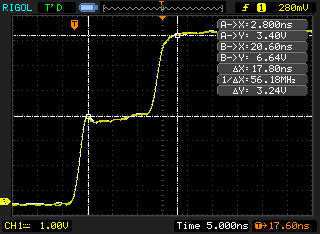
\includegraphics[width=8cm]
			{Imagenes/Res10k.png}
			\caption{Medici\'on para la resistencia de $10k\Omega$. La referencia (en blanco) esta graficada con la l\'inea abierta.}
			\label{img001} 
		\end{figure}

	\indent En la Figura \ref{img002} se muestra el resultado con la 
	resistencia de $1k\Omega$. Puede verse que 
	$$\rho=\frac{Z_L-Z_0}{Z_L+Z_0}$$
	$$\frac{2.96V}{3.40V}=\frac{Z_L- 50\Omega}{Z_L+50\Omega}$$
	
	\indent Por lo tanto $Z_L=722\Omega$, que se corresponde a un valor, si 
	bien aun lejano, m\'as pr\'oximo que en el caso anterior.
		
		\begin{figure}[!htb]
			\centering
			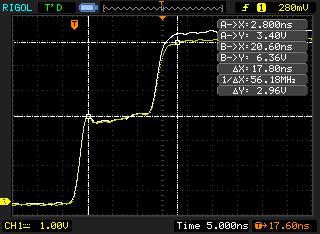
\includegraphics[width=8cm]
			{Imagenes/Res1k.png}
			\caption{Medici\'on para la resistencia de $1k\Omega$. La 
			referencia (en blanco) esta graficada con la l\'inea abierta.}
			\label{img002} 
		\end{figure}

	\indent En la Figura \ref{img003} se muestra el resultado con la 
	resistencia de $120\Omega$. Puede verse que 
	$$\rho=\frac{Z_L-Z_0}{Z_L+Z_0}$$
	$$\frac{1.44V}{3.40V}=\frac{Z_L- 50\Omega}{Z_L+50\Omega}$$
	
	\indent Por lo tanto $Z_L=123\Omega$, el cual es un valor que se encuentra
	dentro del grado de incertidumbre de la resistencia ($120\Omega \pm 10\%$
	para resistores de carb\'on)	

		\begin{figure}[!htb]
			\centering
			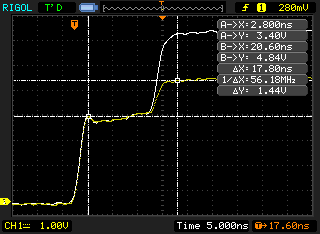
\includegraphics[width=8cm]
			{Imagenes/Res120.png}
			\caption{Medici\'on para la resistencia de $120\Omega$. La 
			referencia (en blanco) esta graficada con la l\'inea abierta.}
			\label{img003}
		\end{figure}
	
	\indent En la Figura \ref{img004} se muestra el resultado con la 
	resistencia de $47\Omega$. Dado su valor cercano a la impedancia 
	caracter\'istica, como era de esperar la onda reflejada es peque\~na. Como
	antes, $$\rho=\frac{Z_L-Z_0}{Z_L+Z_0}$$
	$$\frac{-120mV}{3.48V}=\frac{Z_L- 50\Omega}{Z_L+50\Omega}$$
	\indent Despejando, se obtiene $Z_L=46.6\Omega$, pr\'acticamente 
	coincidiendo con el valor de referencia de $47\Omega$
	
		\begin{figure}[!htb]
			\centering
			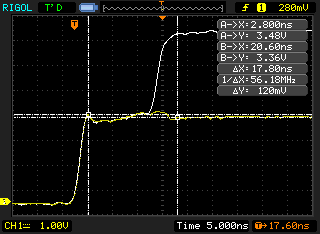
\includegraphics[width=8cm]
			{Imagenes/Res47.png}
			\caption{Medici\'on para la resistencia de $47\Omega$. La 
			referencia (en blanco) esta graficada con la l\'inea abierta.}
			\label{img004}
		\end{figure}

	\indent Por \'ultimo en la Figura \ref{img005}, se realiza la medici\'on 
	con la resistencia de $3.9O\Omega$. Como se puede apreciar es un valor 
	pr\'oximo a un cortocircuito, con lo cual en el gr\'afico se puede 
	observar que el pulso se recorta. Como $$\rho=\frac{Z_L-Z_0}{Z_L+Z_0}$$
	$$\frac{-2.60V}{3.44V}=\frac{Z_L- 50\Omega}{Z_L+50\Omega}$$
	
	\indent Con lo cual $Z_L=6.9\Omega$ y se aleja del un poco del valor 
	$3.9\Omega$ de referencia
		
		\begin{figure}[!htb]
			\centering
			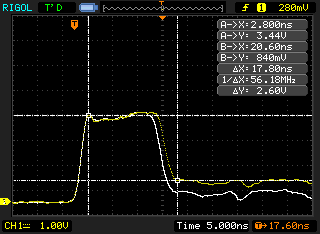
\includegraphics[width=8cm]
			{Imagenes/Res3e9.png}
			\caption{Medici\'on para la resistencia de $3.9\Omega$. La 
			referencia (en blanco) esta graficada con la l\'inea en 
			cortocircuito.}
			\label{img005}
		\end{figure}

	\indent De los resultados obtenidos, cuyo resumen se muestra en la Tabla 
	\ref{tab001}, debe notarse que las mediciones de menor error son aquellas 
	cuya resistencia de carga es cercana a la impedancia caracter\'istica. En
	particular las resistencias mucho mayores a $Z_0$, como la de $10k\Omega$ 
	tienen un error elevado y esto se debe a que para $0\leq \rho \leq 1$ 
	est\'an asociadas resistencias del orden $Z_0 \leq R_L \leq \infty$, con 
	lo cual la exactitud es menor
	
		\begin{table}[!htp]
			\centering
			\begin{tabular}{|c|c|c|c|}
				\hline
    			Valor de referencia & Medici\'on & Error relativo \\
				\hline
				$10k\Omega$ & $2k\Omega$ &$-80 \% $ \\
				\hline 
				$1k\Omega$ & $722\Omega$ &$-27.8\%$\\
				\hline
				$120\Omega$ & $123\Omega$ &$2.5\% $ \\
				\hline
				$47\Omega$ & $46.6\Omega$ &$0.85\% $ \\
				\hline
				$3.9k\Omega$ & $6.9\Omega$ &$76\% $  \\
				\hline								
			\end{tabular}
			\caption{Resumen de los resultados obtenidos para las resistencias
			} 
			\label{tab001}
		\end{table}
		
						
	\subsection{Medición 2 - Bobina}
	\indent En esta secci\'on se pretende medir la inductancia de una bobina y
	su valor de resistencia equivalente serie. El banco de medici\'on es el 
	mismo que el anterior solo que la l\'inea se carga con el inductor. \\
	\indent Cuando el flanco del pulso incidente llegue al inductor, este 
	presentar\'a alta impedancia, con lo cual, inicialmente la respuesta se 
	asemeja a aquella en la que la l\'inea est\'a abierta. La respuesta 
	decaer\'a exponencialmente con $\tau=\frac{L}{Z_0+R_L}$, donde $R_L$ es la
	resistencia serie del inductor, hasta un valor de tensi\'on no nulo que 
	permite conocer el valor de $R_L$ por medio del coeficiente de 
	reflexi\'on. \\
	\indent En la Figura \ref{img006}, se puede observar la respuesta temporal
	cuando se carga la l\'inea con el inductor. Como se esperaba la respuesta
	es exponencial decreciente con 
	$\tau=\frac{L}{Z_0+R_L}=580ns=\frac{L}{50\Omega+R_L}$, con lo cual es 
	necesario conocer el valor de $R_L$, para saber el de $L$.
		
		\begin{figure}[!htb]
			\centering
			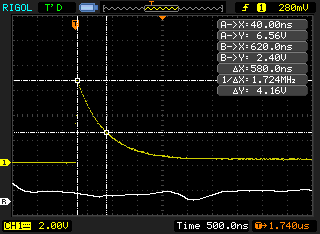
\includegraphics[width=8cm]
			{Imagenes/InductorL.png}
			\caption{Respuesta temporal para la medici\'on de la inductancia 
			de una bobina.}
			\label{img006}
		\end{figure}

	\indent De la Figura \ref{img007} puede hallarse el valor residual de 
	tensi\'on y aplicar la relaci\'on  $\rho=\frac{R_L-Z_0}{R_L+Z_0}$, para 
	obtener la resistencia serie del inductor. De esta manera 
	$$\frac{320mV-3.40V}{3.40V}=\frac{R_L-50\Omega}{R_L-50\Omega}$$
	
	\indent Con lo cual $R_L=2.5\Omega$ y por lo tanto $L=30,45\mu Hy$, el 
	valor que difiere solamente un $1.5\% $ del valor de referencia (
	$L_{ref}=30\mu Hy$).
	
		\begin{figure}[!htb]
			\centering
			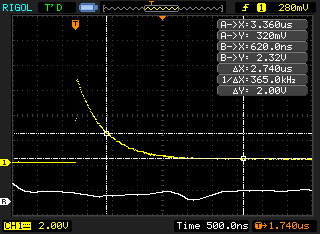
\includegraphics[width=8cm]
			{Imagenes/InductorR.png}
			\caption{Respuesta temporal para la medici\'on de la resistencia 
			equivalente serie de una bobina.}
			\label{img007}
		\end{figure}			
	
	
	\subsection{Medición 3 - Cortocircuito}
	%TODO

	\subsection{Medición 4 - Capacitor}
	\indent En esta medición se utilizaron 3 capacitores distintos para medir
	la resistencia y capacidad equivalente. Los valores utilizados fueron 
	$100pF$, $180pF$ y $47nF$. \\
	\indent La imagen \ref{img010} muestra las respuestas de dichas 
	mediciones. La figura de la izquierda es la respuesta del capacitor de 
	$100pF$, la del medio posee uno de $180pF$ y la de la derecha $47nF$. \\
	
		\begin{figure}[!htb]
			\centering
			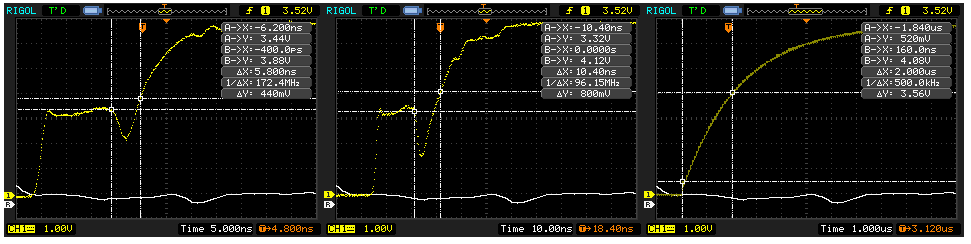
\includegraphics[width=12cm]
			{Imagenes/CurvasCapacitor.png}
			\caption{Respuestas de los distintos capacitores}
			\label{img010} 
		\end{figure}

	\indent Para poder determinar el capacitor y ressitencia equivalente lo 
	primero que se hace es determinar el tiempo de crecimiento $\tau$. El cual
	posee la siguiente fórmula

		\begin{equation}
			\tau = R\cdot C
		\end{equation}
	
	\indent La línea de transmisión posee una impedancia característica de 
	$50\Omega$. Se desprecia la resistencia interna del capacitor. \\
	\indent Despejando el valor de C, en la tabla \ref{tab002} se reflejan los 
	resultados calculados con su respectivas incertidumbres. \\

		\begin{table}[!htp]
			\centering
			\begin{tabular}{|c|c|c|c|c|}
				\hline
    			C teórico & $\tau$ medido & error relativo osciloscopio & C 
				medido &
				$\Delta$C \\
				\hline
				100 pF & $5.8~\text{n seg}$ &  & 120 pF & \\
				\hline 
				180 pF & $10.4~\text{n seg}$ & & 200 pF & \\
				\hline
				47 nF & $2~\mu\text{seg}$ & & 40 nF & \\
				\hline
			\end{tabular}
			\caption{Capacitancias medidas} 
			\label{tab002} %TODO corregir el valor de la tabla y terminar de armarla
		\end{table}

	\newpage
	\section{Colcusiones}
	\indent De las mediciones de resistencias utilizando reflectometría cabe 
	destacar que el valor medidio posee más incertidumbre a medida que el 
	valor de resistencia se aleja de la impedancia característica de la línea.
	%TODO
\end{document}

